\documentclass{beamer}
\usepackage[utf8]{inputenc}
\usepackage{xcolor}
\usepackage{listings}
\usepackage{graphicx}
\usetheme[secheader]{Boadilla}
\definecolor{coultitre}{rgb}{0,0.65,0}
\setbeamercolor{structure}{fg=coultitre, bg=coultitre!40} 



\title{Vidéo surveillance, Streaming vidéo et contrôle de caméra via Android }
\author{\tiny{Jérôme NAHELOU, Quentin NEBOUT, Romain SOLVE, Fabien QUINTARD}}

\institute{\large{Chargé de Projet : Yérom-David Bromberg}\\ \bigskip{}

\small{Université Bordeaux 1}}
\date{29 mars 2011}


\begin{document}
\frame[plain]{\titlepage}

\AtBeginSection[]{
\begin{frame}<beamer>
\frametitle{Plan}
\small{\tableofcontents[currentsection,hideallsubsections]}
\end{frame}}

\begin{frame}
\frametitle{Plan de l'exposé}
\small{\tableofcontents[hideallsubsections]}
\end{frame}


  \begin{frame}
   \frametitle{Description}
  Introduction
  % schéma projet : dessin camera + portablets et tablettes android en réseau %
   \begin{itemize}
    \item Android: OS pour appareil mobile, basé sur noyaux linux
    \item Choix: M-JPEG, HTTP-GET
   \end{itemize}
  \end{frame}
  
  \begin{frame}
   \frametitle{Besoins}
  Introduction
  % schéma besoins F / besoins NF %
  \end{frame}

\section{Aspect général de l'application}
  \subsection{Description}
  \begin{frame}
   \frametitle{Description}
  Aspect général de l'application convivial
   \begin{itemize}
    \item Astuces pour mieux connaître les fonctionnalités
    \item Application Multi-langue avec détection automatique
   \end{itemize}
  \end{frame}

%\section{Simple vue}
%\subsection{Spécifications}
% \begin{frame}
%   \frametitle{Spécifications}
%   \begin{itemize}
%    \item Réutilisation d'un lecteur MJPEG existant : MjpegView
%    \item Interface de contrôle de la caméra
%    % screen simple vue %
%    \end{itemize}
%\end{frame}

%\section{Multi-vue}
%\subsection{Spécifications}
% \begin{frame}
%   \frametitle{Spécifications}
%   \begin{itemize}
%    \item Implémentation de layouts personnalisés pour 2 à 6 caméras
%    % schéma ou screen multi-vue %
%    \item Rafraîchissement multi-threadé (un thread par caméra)
%    % schéma UML de Jérôme ;) %
%    \item Ajout de listeners pour gérer les caméras et passer en simple vue 
%    \end{itemize}
%\end{frame}

%\section{Contrôle de la caméra}
%\subsection{Implémentation}
% \begin{frame}
%   \frametitle{Implémentation}
%   \begin{itemize}
%    \item Communication avec la caméra par requêtes HTTP
%    \item Chargement de la configuration à l'initialisation de la vidéo
%    \item Méthode de construction et d'envoi des requêtes avec
%    authentification et délai variable de connexion
%   \end{itemize}
%\end{frame}

%\subsection{Interfaces}
% \begin{frame}
%\frametitle{Interfaces}
%   Plusieurs interfaces de contrôle direct :
%   \begin{itemize}
%    \item Flux vidéo en continu pour actions en temps réel
%    \item Contrôle du Pan/Tilt/Zoom de manière tactile
%    % schéma notion tactile %
%    \item Interface de commandes avancées adaptée à la caméra
%    \item Module de gestion de détection de mouvements
%   \end{itemize}
%\end{frame}

%\section{Détection de mouvements}
%\subsection{Principe Axis}
% \begin{frame}
%   \frametitle{Pricipe Axis}
%    Le mécanisme de la détection de mouvements par Axis est le suivant :
%   \begin{itemize}
%    \item Ajout d'une fenêtre de détection spécifique (coordonnées,
%    sensibilité, \ldots) par l'utilisateur
%    \item Solution 1 : Ajout d'un événement déclenché automatiquement à la
%    présence d'un mouvement (email, SMS, \ldots)
%    \item Solution 2 : Demande du flux de niveaux de détection pour un
%    calcul et un traitement personnalisés
%   \end{itemize}
%\end{frame}

\subsection{Implémentation Android}
 \begin{frame}
   \frametitle{Implémentation Android}
    La solution 2 a été retenue pour notre application :
    \begin{itemize}
    \item Définition de la fenêtre directement sur l'écran (composant
    graphique)
    \item Mise en arrière-plan du thread de calcul (utilisation d'un service
    Android)
    \item Alerte par notification : vibration + snapshot
    % deuxième schéma UML de Jérôme %
   \end{itemize}
\end{frame}



\section{Gestion des caméras}
  \begin{frame}
   \frametitle{Gestion des caméras}


\begin{figure}[H]
  \centering
  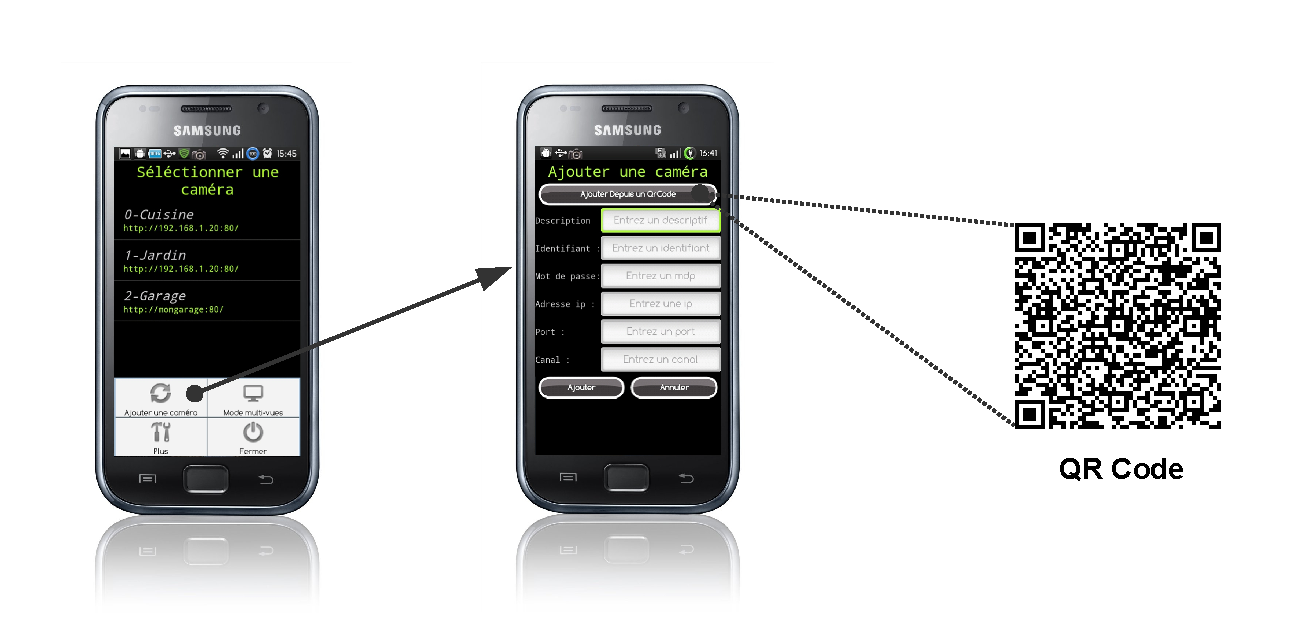
\includegraphics[scale=0.25]{Images/ImageSlide5.pdf}
     \begin{itemize}
    \item Ecran d'accueil de l'application, accès aux différentes activités
    \item Liste illimitée de caméras sauvegardable
    \item Gestion complète des caméras : ajout / édition / suppression
    \item Possiblité d'ajout par QRCode
   \end{itemize}
  \end{figure}  

  \end{frame}


\section{Simple vue}
  \begin{frame}
   \frametitle{Simple vue}


\begin{figure}[H]
  \centering
     \begin{enumerate}
    \item Visualisation de base (contrôle PTZ tactile)
    \item Interface de contrôles avancés
    \item Mode détection de mouvements
   \end{enumerate}
   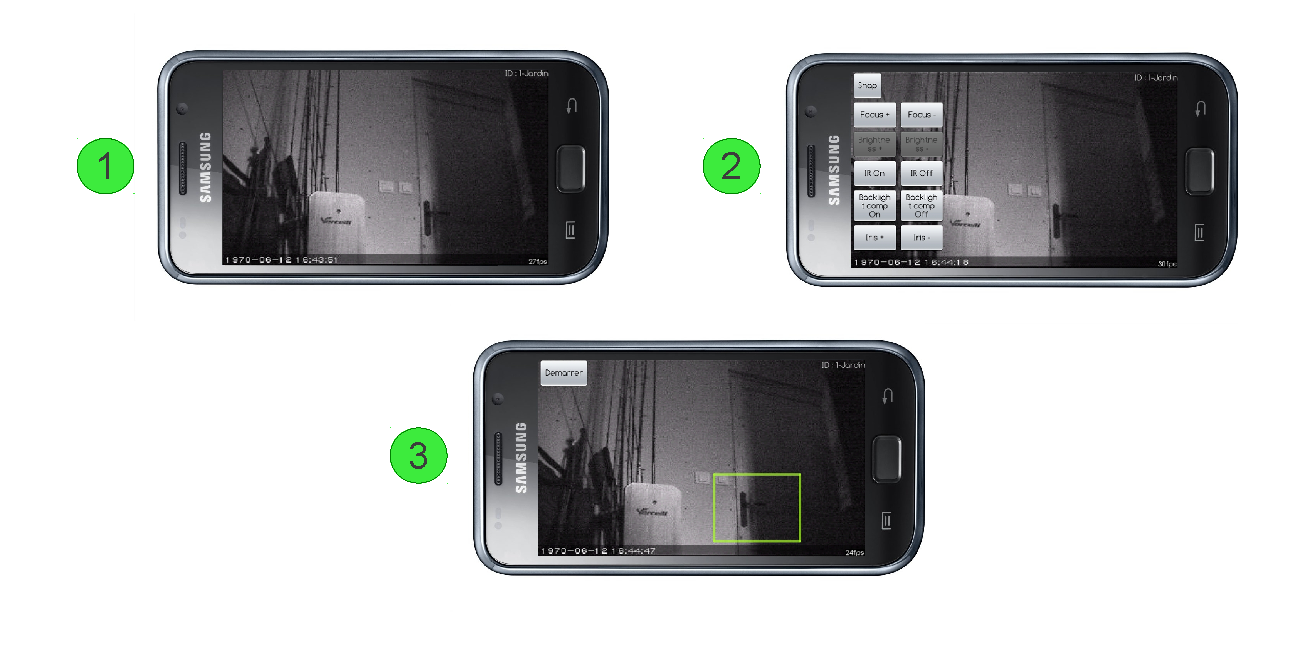
\includegraphics[scale=0.25]{Images/ImageSlide6.pdf}
  \end{figure}  

  \end{frame}

\subsection{Communication avec la caméra}
  \begin{frame}
   \frametitle{Communication et configuration}

  \begin{minipage}{0.94\textwidth}
  \centering
     \begin{itemize}
    \item Classe dédiée au traitement des requêtes HTTP envoyées à la caméra
    \begin{itemize}
      \item Codes réponses divers
      \item Parsage si nécessaire
      \newline
    \end{itemize}
    \item Chargement de la configuration et des fonctionnalités supportées
    \begin{itemize}
      \item PTZ, focus, iris, luminosité, \ldots
      \item Mode auto, résolutions d'images
      \item Audio, détection de mouvements
      \newline
    \end{itemize}
    \item Adaptation de l'interface aux différents modèles de caméra Axis
    \begin{itemize}
      \item Etat des boutons
      \item Choix de la résolution pour la capture
      \newline
    \end{itemize}
   	\end{itemize}
  \end{minipage}

  \end{frame}


\section{Contrôle PTZ tactile}
  \begin{frame}
   \frametitle{Contrôle PTZ tactile}


\begin{figure}[H]
  \centering
    \begin{itemize}
      \item Gestion du déplacement de la caméra (Pan/Tilt) avec 1 pointeur
      (1)
      \item Gestion du zoom avec 2 pointeurs (2)
      \item Réglage de la sensibilité dans les paramètres
   	\end{itemize}
   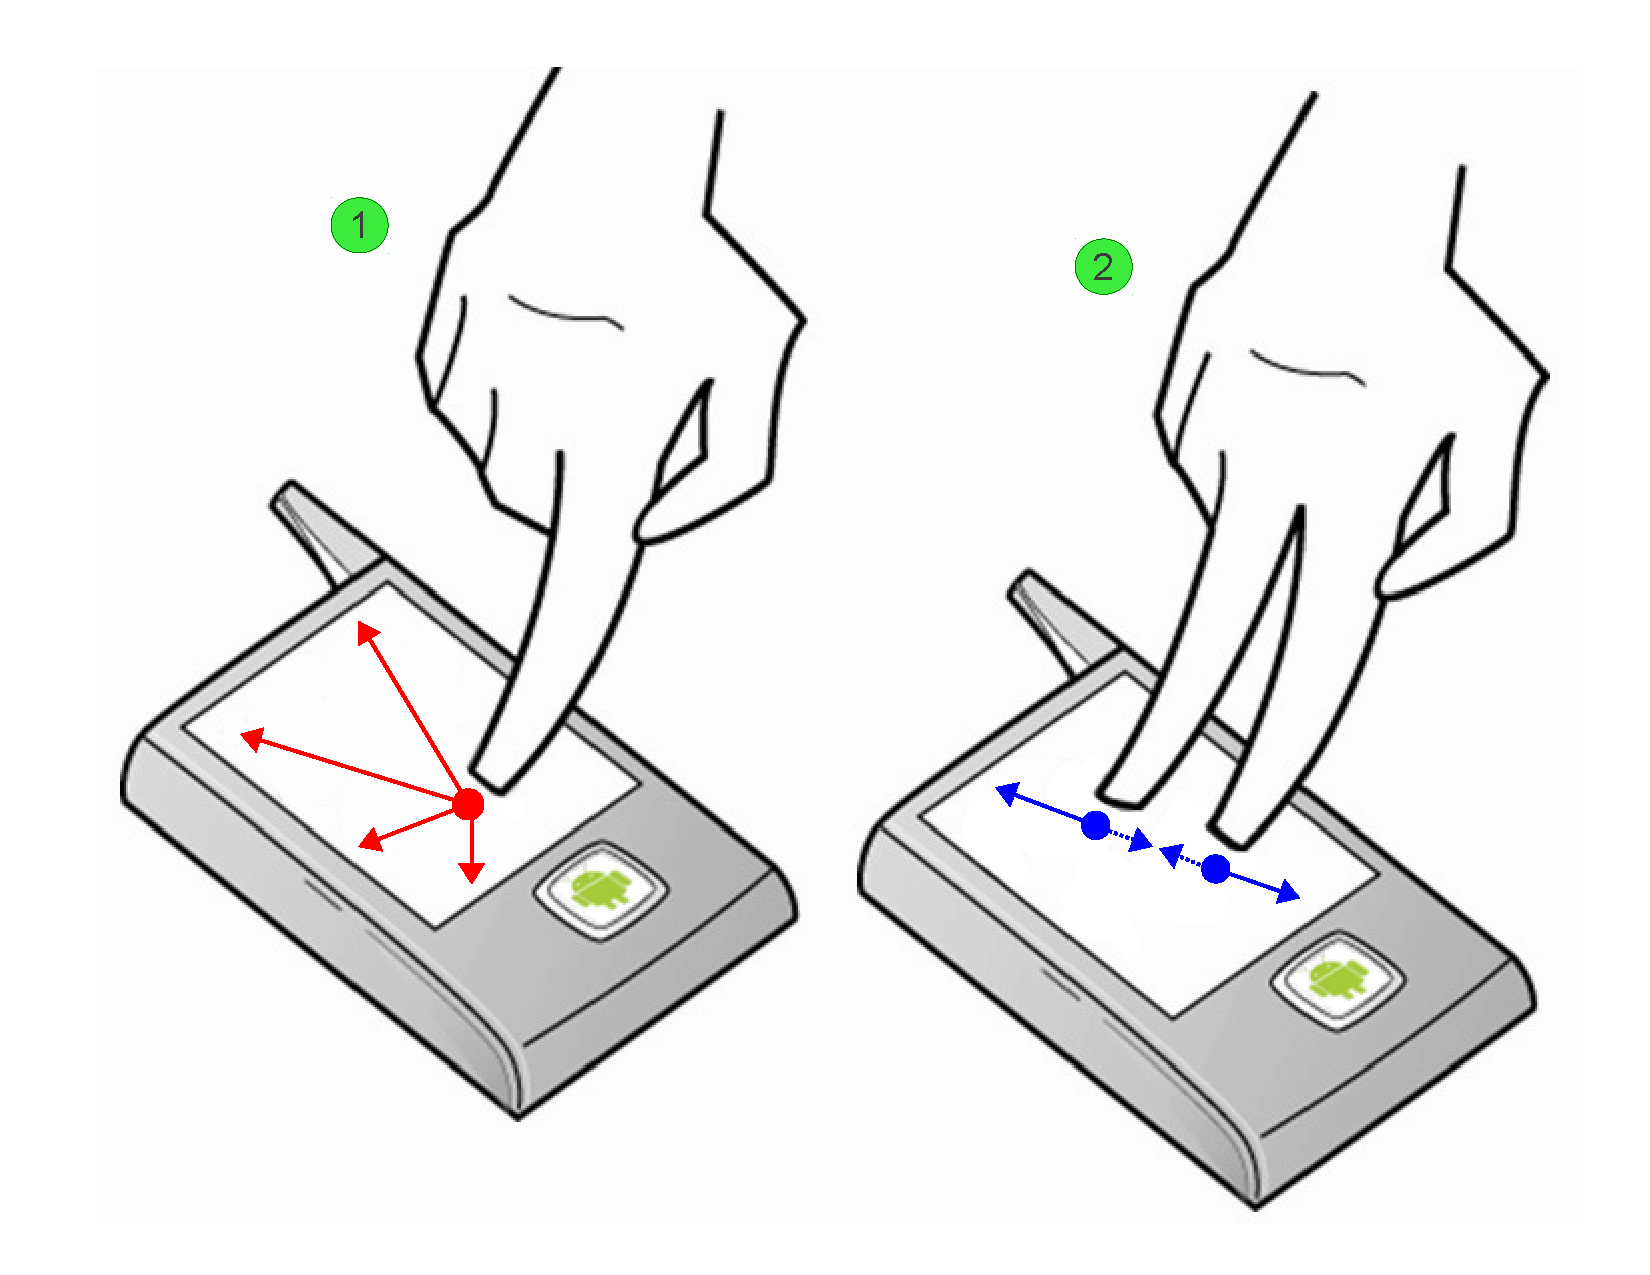
\includegraphics[scale=0.25]{Images/ImageSlide8.pdf}
  \end{figure}  

  \end{frame}


\section{Vue Multiple}
  \subsection{Analyse du besoin}
  \begin{frame}
   \frametitle{Analyse du besoin}


\begin{figure}[H]
  \centering
  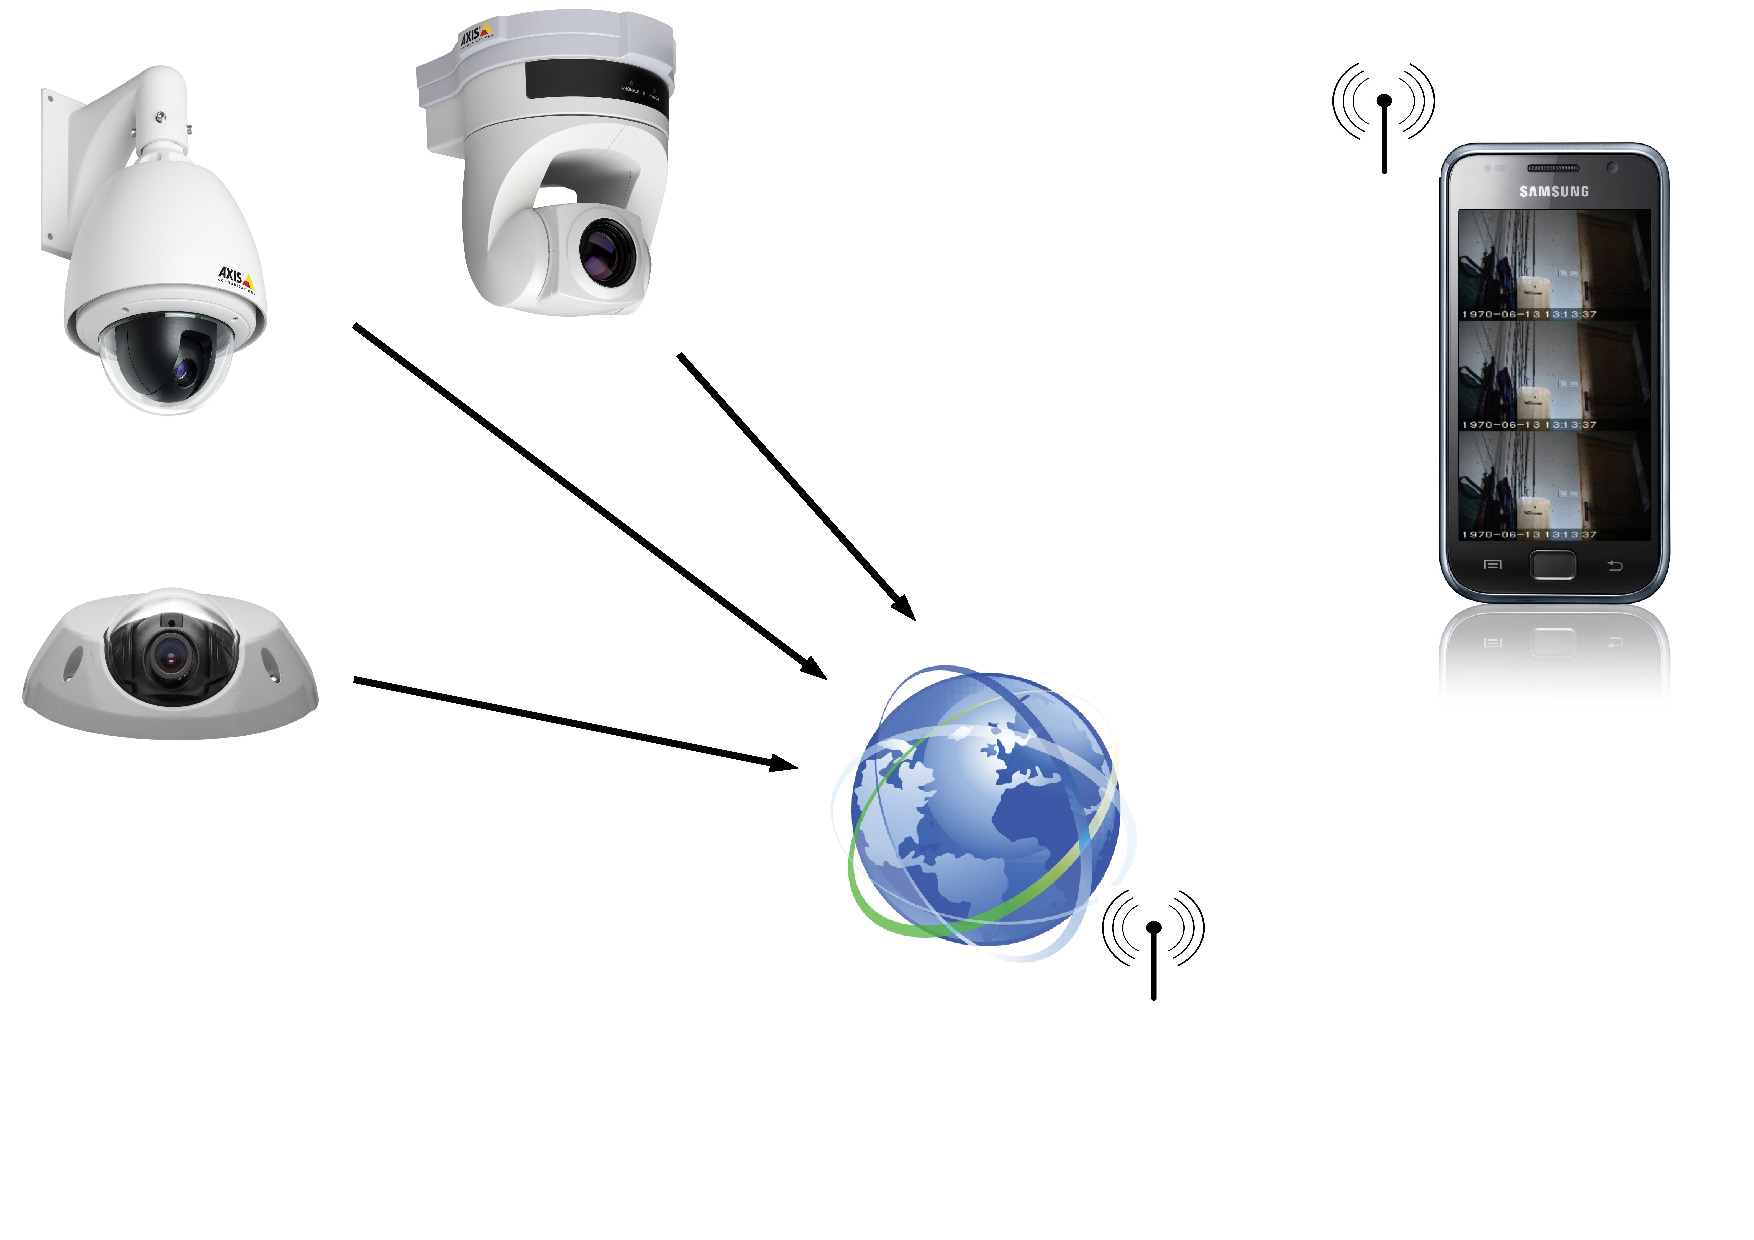
\includegraphics[scale=0.25]{Images/ImageSlide9.pdf}
     \begin{itemize}
    \item Possibilité de visionner 1 à 6 Caméras simultanément
    \item Choix de la disposition des caméras par l'utilisateur
    \item Réglage du nombre d'images par seconde
    \item Switch ``Multiple-Vue" - ``Vue unitaire"
   \end{itemize}
  \end{figure}  

  \end{frame}

  \subsection{Implémentation}
  \begin{frame}
   \frametitle{Implémentation}




  \end{frame}


\section{Détection de mouvement}
 \subsection{Analyse du besoin}
  \begin{frame}
   \frametitle{Détection des mouvements :}



\begin{columns}
\begin{column}{5cm}

   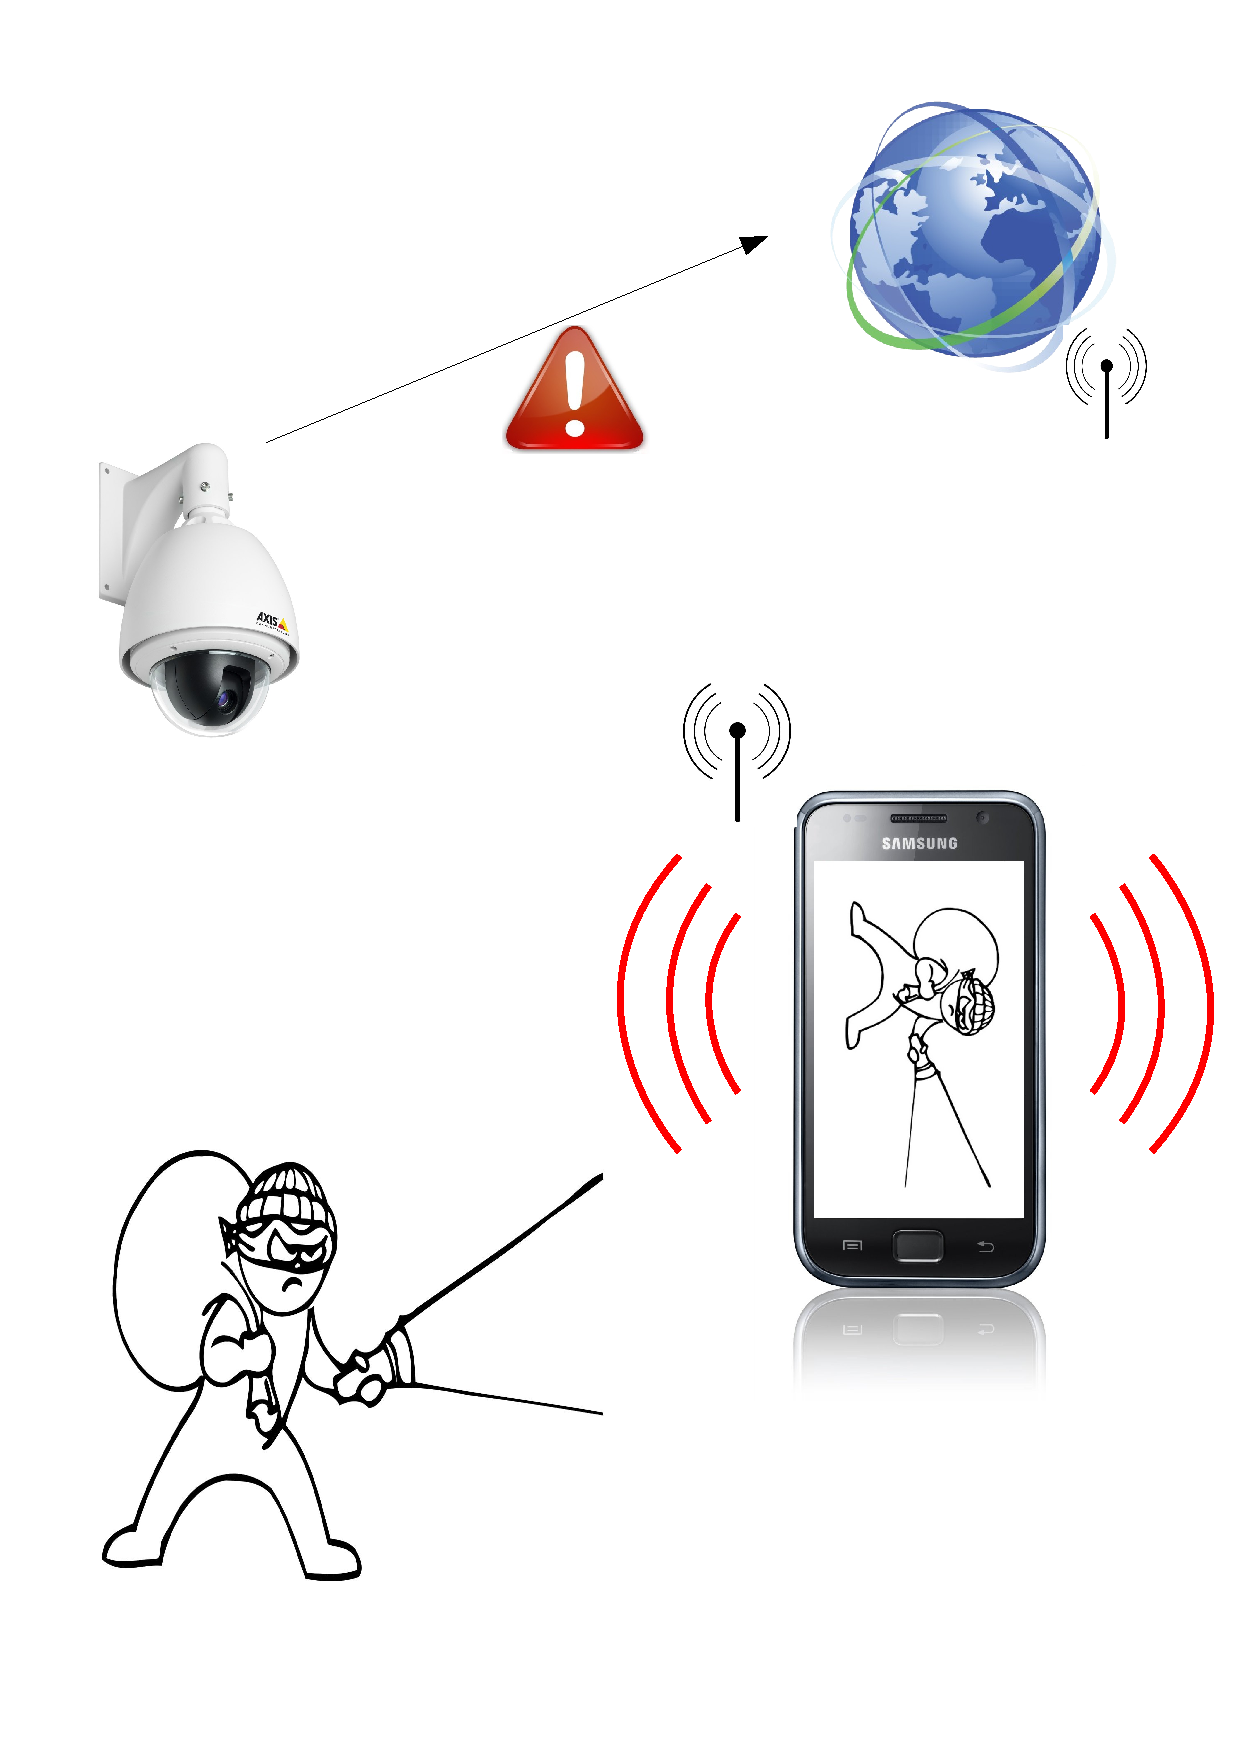
\includegraphics[scale=0.25]{Images/ImageSlide10.pdf}
\end{column}
\begin{column}{7cm}
\textbf{\textit{Caractéristiques :}} 
\begin{itemize}
    \item Réglage de la fenètre et du seuil de détection.
  	\item 1 à 10 fenètres par caméra.
  	\item Détection illimitée pour des caméras differente.
 	\item Notification via Vibration et Cliché instantanné.
 	\item Utilisation facile et intuitive.
\end{itemize}
\end{column}
\end{columns}
  \end{frame}

  \subsection{Implémentation}
  \begin{frame}
   \frametitle{Implémentation}

  \end{frame}

  
\subsection{Extras}
\begin{frame}
\frametitle{Extras}
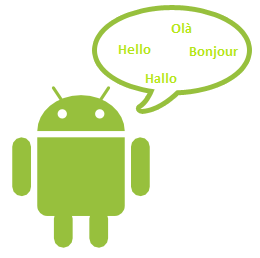
\includegraphics[width=3cm, height=2.5cm]{Images/ImageSlide11-3.png}\\
\begin{minipage}{0.69\textwidth}
\begin{itemize}
  \item Application Multi-langues
  \item Astuces au démarrage
  \item Snapshot
  \item Partage de l'application et des caméras
  \item Import-export de la configuration
\end{itemize}
\end{minipage}
\begin{minipage}{0.29\textwidth}
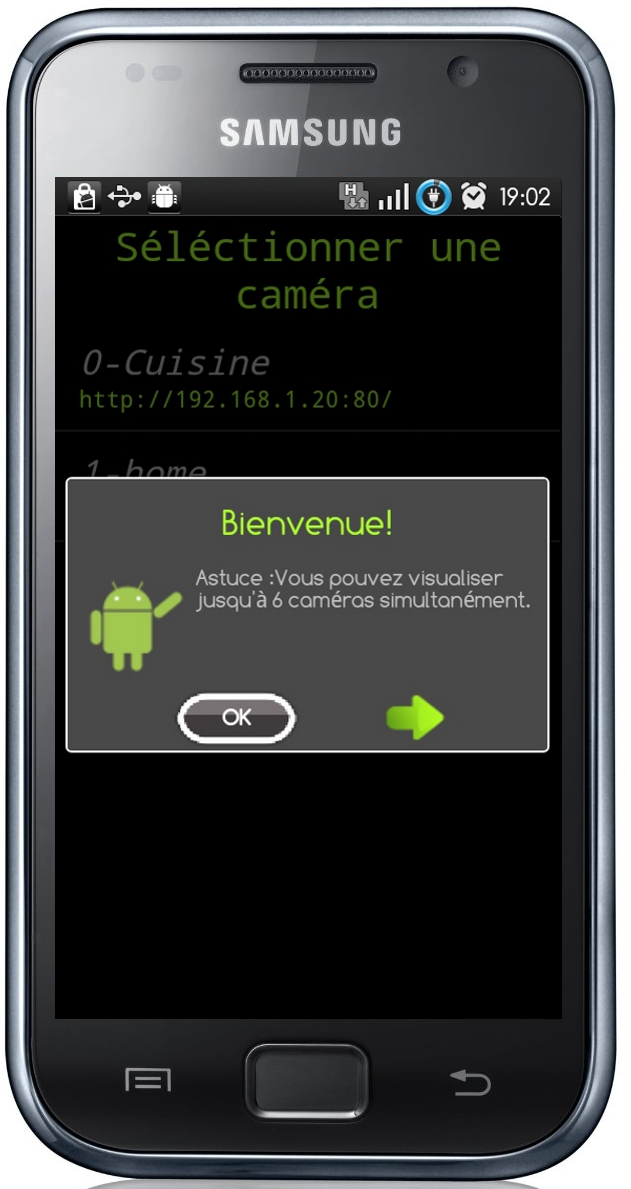
\includegraphics[width=2.5cm, height=4.5cm]{Images/ImageSlide11-3a.png}
\end{minipage}
\end{frame}
\section{Tests Unitaires}
\subsection{Principe}
  \begin{frame}
\begin{minipage}{0.59\textwidth}
\frametitle{Tests Unitaires}
Rôle des tests unitaires
  \begin{itemize}
 \item Garantir le bon fonctionnement de l'application
    \item Vérifier si les fonctions terminent bien
    \item Identifier étape par étape les erreurs éventuelles
\end{itemize} 
\end{minipage}
\begin{minipage}{0.39\textwidth}
 
\includegraphics[width=4cm, height=3.2cm]{Images/ImageSlide12.png}
\end{minipage}
\end{frame}
\subsection{Tests en réel}
 \begin{frame}
\begin{minipage}{0.59\textwidth}
   \frametitle{Tests en réel}
\begin{itemize}
    \item Suivi de l'exécution en continu avec le LogCat d'Android
    \item Utilisation intensive de 3 téléphones de marques différentes
    \item Tests sur une caméra Axis PTZ 214 avec l'ensemble des
    fonctionnalités implémentées
   \end{itemize}
\end{minipage}
\begin{minipage}{0.39\textwidth}
 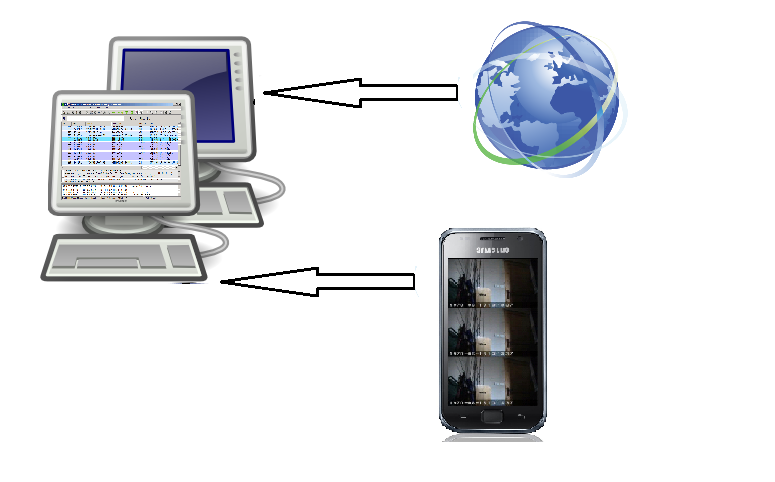
\includegraphics[width=4cm, height=3cm]{Images/ImageSlide13.png}
\end{minipage}
\end{frame}
  \begin{frame}
   \frametitle{Conclusion}
 \begin{itemize}
    \item Cahier des charges : Absence de son
    \item Application testée et opérationnelle
   \end{itemize}
   \begin{figure}[H]
    \centering
\includegraphics[width=2cm, height=2cm]{Images/ImageSlide14.png}
    \end{figure}
\end{frame}


\end{document}